\section{Monkey Testing}
\label{sec:Monkey Testing}

\index{Monkey Testing}A metaphor for naming the producer of any input for a program.

The name 'monkey' comes from the the 'Infinite monkey'\footnote{\url{http://en.wikipedia.org/wiki/Infinite_monkey_theorem}} theorem. There is an adage that ‘\textit{thousand monkeys at a thousand typewriters will eventually type out the entire works of \index{William Shakespeare}Shakespeare}’.

\begin{figure}[!h]
\centering
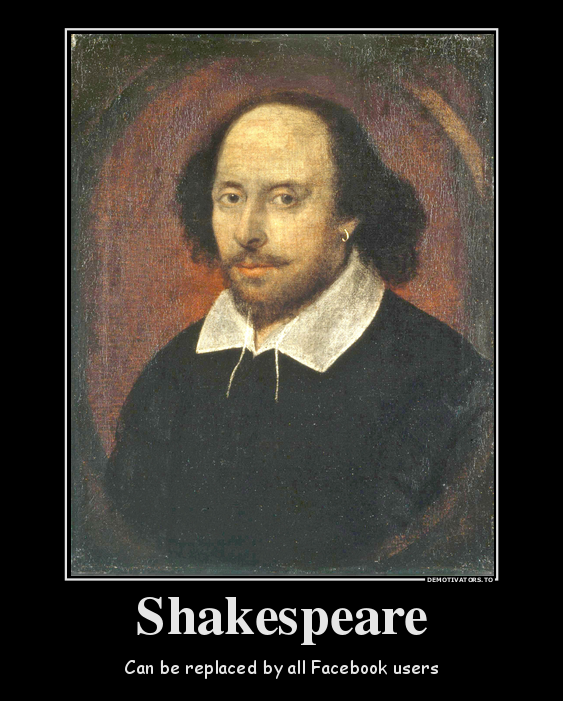
\includegraphics[width=0.8\linewidth]{shakespeare}
\caption{\ttfamily{This is Shakespeare. He looks at you as at an infinite monkey}}
\label{fig:shakespeare}
\end{figure}

For example, a monkey test can enter random strings into text boxes to ensure handling of all possible user input or provide garbage files to check for loading routines that have blind faith in their data. The test monkey is technically known to conduct \index{Random Testing}Random testing.